\input{head.inc}
  
% Präambelbefehle für die Präsentation
\title[TET: Elektromagnetische Wellen V - Wellenpakete]{Elektromagnetische Wellen V - Wellenpakete}

\begin{document}
% 
% Frontmatter 
% 
%%%%%%%%%%%%%%%%%%%%%%%%%%%%%%%%%%%%%%%%%%%%%%%%%%%%%%%%%%%%%%%%%%%%%%%%%%%%%%%%%%%%%%%%%%%%%%%%%%%%%%%%%%%%%%%%%%%%%%%%%%%%% 

%% inserts the title page and the table of contents
\maketitle

% 
% Content 
% 
%%%%%%%%%%%%%%%%%%%%%%%%%%%%%%%%%%%%%%%%%%%%%%%%%%%%%%%%%%%%%%%%%%%%%%%%%%%%%%%%%%%%%%%%%%%%%%%%%%%%%%%%%%%%%%%%%%%%%%%%%%%%% 
\section{Elektromagnetische Wellen V - Wellenpakete}

\begin{frame}
  \frametitle{Ausgangspunkt}
  \begin{itemize}[<+->]
  \item Wir suchen Lösungen der homogenen Wellengleichung
    \begin{equation*}
      \square \Psi(\Ortsr[v], t) = \left(\laplace - \varepsilon\mu\frac{\d^2}{\d t^2}  \right) \Psi(\Ortsr[v], t)
    \end{equation*}
  \item Lösungen, die sich nur in einer Richtung (aber hin- und rücklaufend) ausbreiten, haben die allgemeine Form
    \begin{equation*}
      \Psi (\Ortsr[v], t) = \sum_\omega \left( \Psi_+ (\omega t + \Wellenzahl[v]\cdot\Ortsr[v]) + \Psi_- (\omega t - \Wellenzahl[v]\cdot\Ortsr[v]) \right) \pointspace ; \pointspace \Geschwindigkeit_p =\frac{\omega}{k} \stackrel{\text{hier}}{=} \Geschwindigkeit_c = \frac{1}{\sqrt{\varepsilon\mu}}  
    \end{equation*}
  \item Eine alternative Schreibweise betrachtet die Überlagerung für verschiedene Wellenvektoren \(\Wellenzahl[v] = \Wellenzahl\; \einheitsvek{k} = \omega\sqrt{\varepsilon\mu}\;\einheitsvek{k}\)
    \begin{equation*}
      \boxed{\Psi (\Ortsr[v], t) = \int\limits_{0}^\infty \left[ A_+(k) \Psi_+ (\omega t + \Wellenzahl[v]\cdot\Ortsr[v]) + A_-(k) \Psi_- (\omega t - \Wellenzahl[v]\cdot\Ortsr[v]) \right] \upd \Wellenzahl} \text{ \alert{polychromatische Welle}} 
    \end{equation*}
    \item oBdA: \(\Wellenzahl[v] = \Wellenzahl \einheitsvek{z}   \to \Wellenzahl[v]\cdot\Ortsr[v] = \Wellenzahl z \to\) Ausbreitung entlang \(z\)-Richtung
\end{itemize}
  \end{frame}

\begin{frame}
  \frametitle{Dispersion}
 % \begin{block}{Dispersion}
  \begin{itemize}[<+->]
  \item In der Regel sind die Materialparameter \alert{frequenzabhängig}:
    \begin{align*}
      \varepsilon &= \varepsilon_0\varepsilon_r = \varepsilon_0\varepsilon_r(\omega) & \mu &= \mu_0\mu_r = \mu_0\mu_r(\omega)  
    \end{align*}
  \item Somit haben \alert{Teilwellen unterschiedliche Phasengeschwindigkeiten}:
    \begin{equation*}
      \Geschwindigkeit_p (\omega) = \Geschwindigkeit_c(\omega) = \frac{1}{\sqrt{\varepsilon\mu}} = \frac{1}{\sqrt{\varepsilon_0\mu_0}} \frac{1}{\sqrt{\varepsilon_r(\omega)\mu_r(\omega)}}=\frac{c}{n(\omega)} 
    \end{equation*}
  \item Dies tritt insbesondere bei \alert{Wellenpaketen} in Erscheinung
  \end{itemize}
%\end{block}
  \end{frame}

  
\begin{frame}
  \frametitle{Wellenpaket}
  %\begin{block}{Wellenpaket}
      \begin{itemize}[<+->]
    \item Unter einem Wellenpaket mit \alert{harmonischer Zeitabhängigkeit}, das in \alert{\(+z\)-Richtung} propagiert, versteht man eine Überlagerung der Form
    \begin{equation*}
      \Psi (\Ortsr[v], t) = \int\limits_{-\infty}^\infty \underline{A(k)} \euler^{\komplex (\omega t - \Wellenzahl z)} \upd \Wellenzahl\; , \text{ mit } \underline{A}(-k) = \underline{A}^\star(k)
    \end{equation*}
    \item Häufiger Spezialfall: $\underline{A}(k) = A(k)$ reelwertig mit $A(-k) = A(k)$
  \item Hierbei soll \(A(k)\) zunächst \alert{konzentriert} sein um \(\Wellenzahl = \Wellenzahl_0\): 

    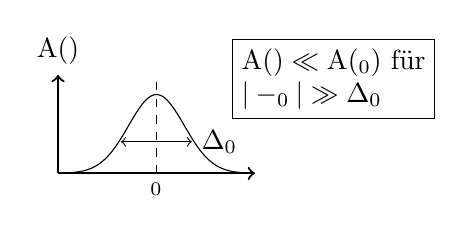
\begin{tikzpicture}[scale=0.5, samples=200, domain=0:5]
	% Achsen zeichnen
	\draw[->,thick] (0,0) -- (5,0) node[right] {$\Wellenzahl$};
	\draw[->,thick] (0,0) -- (0,2.5) node[above] {$\mathrm{A}(\Wellenzahl)$};
	%Plot
	\draw plot (\x,{exp(-(\x-2.5)^2)*2});
	\draw [style=dashed] (2.5,0) node[below] {$\Wellenzahl_0$} --(2.5,2.4);
	\draw[<->] (1.6,.8)--(3.4,.8) node[right] {$\Delta \Wellenzahl_0$};
	\node[draw,align=left] at (7,2.4) {$\mathrm{A}(\Wellenzahl) \ll \mathrm{A}(\Wellenzahl_0)$ für\\ $|\Wellenzahl-\Wellenzahl_0| \gg \Delta \Wellenzahl_0$};
\end{tikzpicture}
    \end{itemize}
    %\end{block}
  \end{frame}



 \begin{frame}
  \frametitle{Taylor-Entwicklung von \(\omega(\Wellenzahl)\)}
      \begin{itemize}[<+->]
      \item Da die Wichtungsfunktion \(A(\Wellenzahl)\) um \(\Wellenzahl = \Wellenzahl_0\) konzentriert ist, bietet sich eine \alert{Taylorentwicklung} von \(\omega(\Wellenzahl)\) um \(\Wellenzahl_0\) an:
\begin{align*}
\omega(\Wellenzahl) &= \omega(\Wellenzahl_0) + \left.\frac{\upd \omega}{\upd \Wellenzahl}\right|_{\Wellenzahl_0} (\Wellenzahl - \Wellenzahl_0) + \ldots\\
&\cong \underbrace{\omega(\Wellenzahl_0)}_{=\omega_0} + \Geschwindigkeit_{\mathrm{g}}(\Wellenzahl-\Wellenzahl_0) &\rightarrow\boxed{\Geschwindigkeit_{\mathrm{g}} = \left.\frac{\upd \omega}{\upd \Wellenzahl}\right|_{\Wellenzahl_0}}\text{ \alert{Gruppengeschwindigkeit}\hspace*{2cm}}
\end{align*}
\item Verlauf von \(\omega(\Wellenzahl)\) (\alert{Dispersionsrelation}) mit und ohne Dispersion

  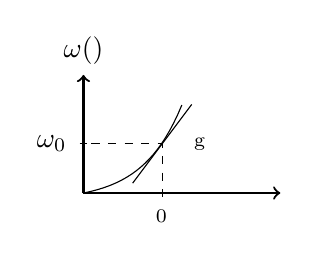
\begin{tikzpicture}[scale=0.5,domain=0:2.5]
	% Achsen zeichnen
	\draw[->,thick] (0,0) -- (5,0) node[right] {$\Wellenzahl$};
	\draw[->,thick] (0,0) -- (0,3) node[above] {$\omega(\Wellenzahl)$};
	%Plot
	\draw plot (\x,{0.2*exp(\x)-0.2});
		% Beschriftung
	\draw (-.1,1.25) -- (.1,1.25) node[left=4pt] {$\omega_0$};
	\draw (2,-.1) -- (2,.1) node[below=4pt] {$\Wellenzahl_0$};
	\draw[style=dashed] (.2,1.25)--(2,1.25) node[right=8pt] {$\Geschwindigkeit_{\mathrm{g}}$} -- (2, .2);
	\draw (1.25,0.25)--(2.75,2.25);
\end{tikzpicture}
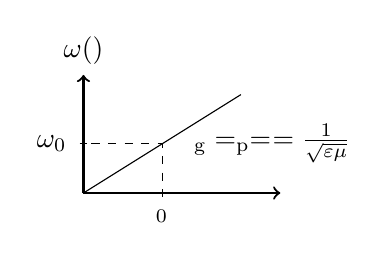
\begin{tikzpicture}[scale=0.5]
	% Achsen zeichnen
	\draw[->,thick] (0,0) -- (5,0) node[right] {$\Wellenzahl$};
	\draw[->,thick] (0,0) -- (0,3) node[above] {$\omega(\Wellenzahl)$};
	% Plott
	\draw (0,0) -- (4,2.5);
	% Beschriftung
	\draw (-.1,1.25) -- (.1,1.25) node[left=4pt] {$\omega_0$};
	\draw (2,-.1) -- (2,.1) node[below=4pt] {$\Wellenzahl_0$};
	\draw[style=dashed] (.2,1.25)--(2,1.25)node[right=8pt] {$\Geschwindigkeit_{\mathrm{g}}=\Geschwindigkeit_{\mathrm{p}}=\Geschwindigkeit_{\lichtgeschw} = \frac{1}{\sqrt{\varepsilon\mu}}$} -- (2, .2);
\end{tikzpicture}
\end{itemize}
  \end{frame}
 
         \begin{frame}
           \frametitle{TET-Einführung \(\to\) Beiträge zum komplexen \(\varepsilon\)}
           \begin{columns}[t]
             \begin{column}{.6\textwidth}
               
               \centering
               \onslide<+->{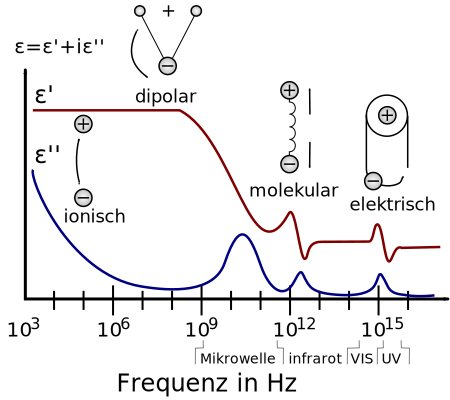
\includegraphics[width=\columnwidth]{Dielectric_responses_DE.png}
               {\tiny Quelle:  Prof. Kenneth A. Mauritz, derivative work: Cepheiden, Attribution, via Wikimedia Commons}}
             \end{column}
             \begin{column}{.4\textwidth}
               \begin{itemize}
                 \item Grundsätzlich verschiedenes Verhalten bei
                   vorhandenen oder nicht vorhandenen Rückstellkräften
                   \item dipolar: Polare Moleküle (z.B. Wasser)
                     orientieren sich im Feld, keine Rückstellkraft
                     (nur thermische Bewegung) $\to$ Debye-Relaxation
                     \item molekular, atomar: Rückstellkräfte
                       vorhanden $\to$ harmonischer Oszillator
                       \item Dielektrische Spektroskopie $\to$
                         Aufklärung der Mechanismen
                 \end{itemize}
             \end{column}
           \end{columns}
         \end{frame}


 \begin{frame}
  \frametitle{Taylor-Entwicklung für das Wellenpaket}
      \begin{itemize}[<+->]
      \item Taylor-Entwicklung in e-Funktion einsetzen:
        \begin{equation*}
          \euler^{\komplex (\omega t - \Wellenzahl z)} \cong \euler^{\komplex(\omega_0 t - \Wellenzahl_0 z)} \euler^{\komplex (\overbrace{\Wellenzahl - \Wellenzahl_0}^{=q})(\Geschwindigkeit_{\mathrm{g}} t - z)}
        \end{equation*}
        \item Damit folgt für das Wellenpaket:
        \begin{align*}
\Psi (\Ortsr[v], t) &\cong \underbrace{\int\limits_{-\infty}^{\infty} \underbrace{A(\Wellenzahl_0 + q)}_{A(\Wellenzahl)}\euler^{\komplex q (\Geschwindigkeit_{\mathrm{g}} t - z)}\upd q}_{\mathrm{H}(\Geschwindigkeit_{\mathrm{g}} t -z)} \cdot\; \euler^{\komplex ( \omega_0 t - \Wellenzahl_0 z)}\\
& \cong \underbrace{\mathrm{H}(\Geschwindigkeit_{\mathrm{g}} t -z)}_{\substack{\text{Einhüllende}\\ \text{propagiert mit }\Geschwindigkeit_{\mathrm{g}}\\ \text{in Richtung $z$}}}\cdot\; \underbrace{\euler^{\komplex (\omega_0 t - \Wellenzahl_0 z)}}_{\substack{\text{ebene Welle,}\\ \omega = \omega_0\\ \Wellenzahl = \Wellenzahl_0}}
\end{align*}

 \end{itemize}
  \end{frame}

 \begin{frame}
  \frametitle{Träger und Form des Wellenpakets}

  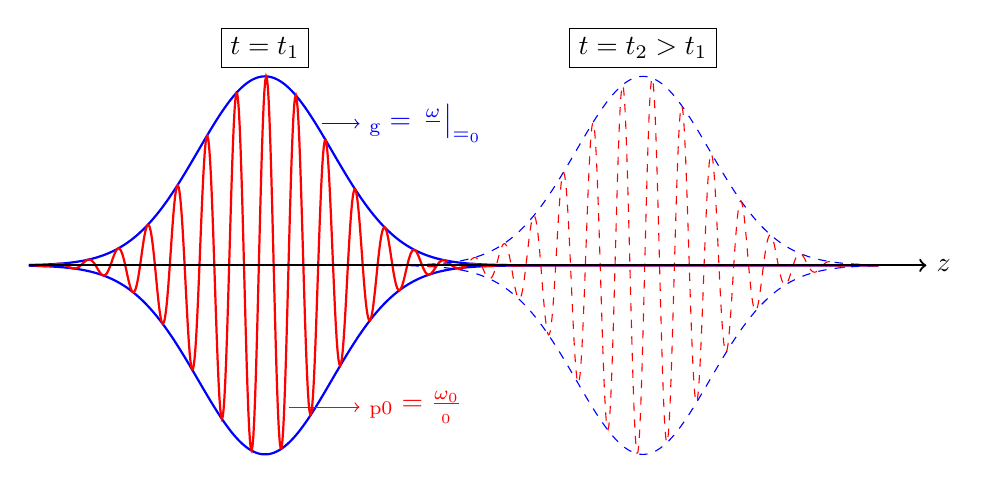
\begin{tikzpicture}[scale=1.2, samples=1000, domain=0:9]
	%Plotten
	\draw [color=blue, thick] plot (\x,{exp(-(\x-2.5)^2)*2}); 
	\draw [color=blue, thick] plot (\x,{-exp(-(\x-2.5)^2)*2});
        \draw [color=red, thick] plot (\x,{cos(deg(\x*20))*exp(-(\x-2.5)^2)*2}); 

	\draw [style=dashed, color=blue] plot (\x,{exp(-(\x-6.5)^2)*2}); 
	\draw [style=dashed, color=blue] plot (\x,{-exp(-(\x-6.5)^2)*2});
        \draw [style=dashed, color=red] plot (\x,{cos(deg(\x*20))*exp(-(\x-6.5)^2)*2}); 

	%\draw[color=red] (0.5,0) sin(0.7,0.5) cos(0.9,0) sin(1.1,-0.66) cos(1.3,0) sin(1.5,1) cos(1.7,0) sin(1.9,-1.37) cos(2.1,0) sin(2.3,1.8) cos(2.5,0) sin(2.7,-2.15) cos(2.9,0) sin(3.1,2.38) cos(3.3,0) sin(3.5,-2.5) cos(3.7,0) sin(3.9,2.38) cos(4.1,0) sin(4.3,-2.15) cos(4.5,0) sin(4.7,1.8) cos(4.9,0) sin(5.1,-1.37) cos(5.3,0) sin(5.5,1) cos(5.7,0) sin(5.9,-0.66) cos(6.1,0) sin(6.3,0.5) cos(6.5,0);
    %\draw (0.5,0.5) cos(2,1.5) sin(3.5,2.5) cos(5,1.5) sin(6.5,0.5);% cos (8,0);
    %\draw (0.5,-0.5) cos(2,-1.5) sin(3.5,-2.5) cos(5,-1.5) sin(6.5,-0.5);% cos (8,0);
   % \begin{axis}
   %        \addplot[samples=500,domain=0:180]{sin(x)*2*sin(20*x)};%x in degrees, 500 samples into the domain
   % \end{axis}
   
   %Beschriftung
   \draw[->, color=blue] (3.1,1.5)--(3.5,1.5) node[right] {$\Geschwindigkeit_{\mathrm{g}}=\left.\frac{\upd \omega}{\upd \Wellenzahl}\right|_{\Wellenzahl=\Wellenzahl_0}$};
   \draw[->, color=red] (2.75,-1.5)--(3.5,-1.5) node[right] {$\Geschwindigkeit_{\mathrm{p0}}=\frac{\omega_0}{\Wellenzahl_0}$};
    \node[draw] at (2.5,2.3) {$t=t_1$};   
    \node[draw] at (6.5,2.3) {$t=t_2>t_1$};   
	% Achse zeichnen
	\draw[->,thick] (0,0) -- (9.5,0) node[right] {$z$};
\end{tikzpicture}
\end{frame}

 \begin{frame}
  \frametitle{Dispersion eines Wellenpakets}
      \begin{itemize}[<+->]
      \item Wir hatten die Dispersionsrelation \(\omega(\Wellenzahl)\) um \(\omega_0\) nach Taylor bis zur ersten Ordnung entwickelt (\alert{linearisiert}) und so das Wellenpaket mit Einhüllender und Träger erhalten.
        \item Aus der Herleitung klar: nur sinnvoll, wenn \(A(k)\) um \(k_0\) \alert{konzentriert} ist.
        \item Bei breitbandiger Überlagerung: Das Wellenpaket enthält viele Frequenzanteile, die in der Regel alle mit \alert{unterschiedlicher Phasengeschwindigkeit} \(\Geschwindigkeit_p(\omega)\) propagieren.
        \item Hierdurch verändert sich die Form der Einhüllenden. Auch dies wird häufig \alert{Dispersion} genannt.
          \item Dieses \alert{Zerfließen} eines Wellenpakets (Signals) ist eine wichtige Begrenzung beim technischen Einsatz (z.B. Signalübertragung über lange Distanzen in Glasfaser-Kabeln)
 \end{itemize}
  \end{frame}

 \begin{frame}
   \frametitle{Dispersion eines Wellenpakets (Beispiel)}
   \centering
   \includegraphics[width=.85\textwidth]{puls-disp}
  \end{frame}


\input{finalframe.inc}
   
\end{document}